\part{NES hardware}
\frame{\partpage}

\begin{frame}{Nintendo Entertainment System (NES)}
	\begin{columns}
		\begin{column}{0.32\textwidth}
			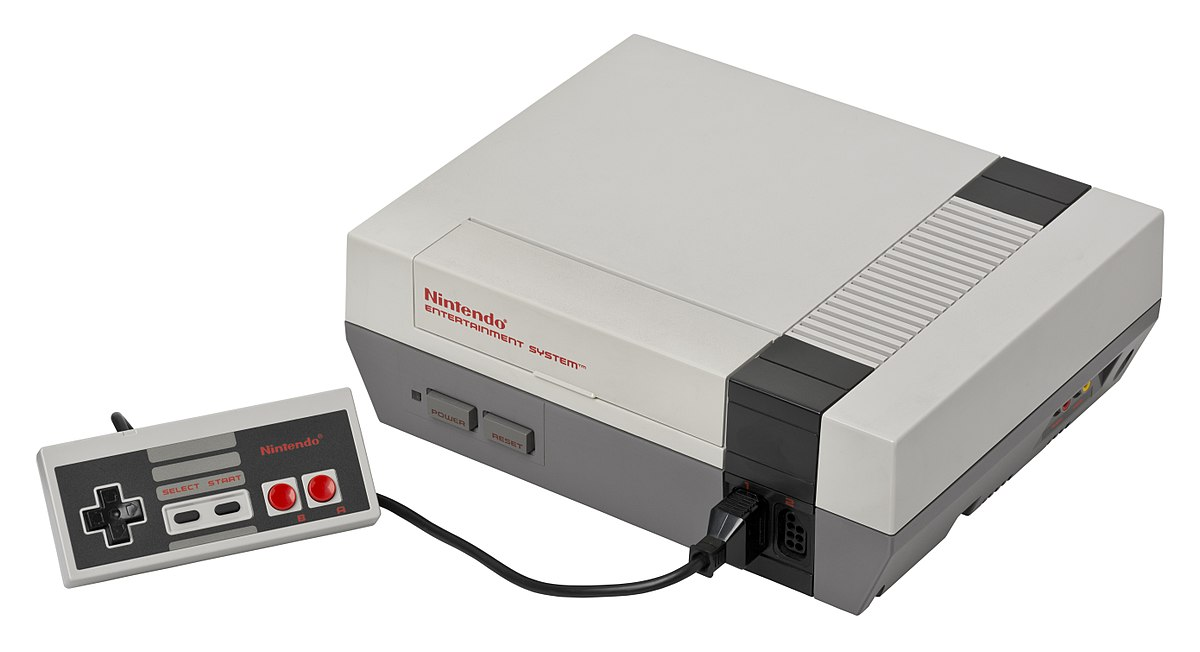
\includegraphics[width=\textwidth]{nes}
			
			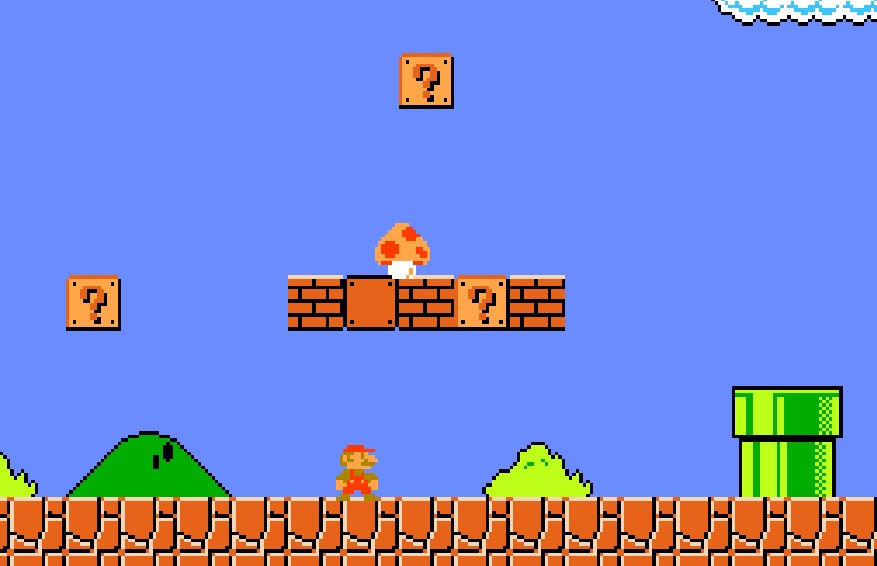
\includegraphics[width=\textwidth]{supermario}
		\end{column}
		\begin{column}{0.64\textwidth}
			\begin{itemize}
				\pause\item Released in \textbf{1983}
				\pause\item Sold as the \textbf{Famicom} (Family Computer) in Japan
				\pause\item Nearly \textbf{62 million} units sold worldwide
				\pause\item Biggest selling game: \textbf{Super Mario Bros}
				\pause\item Credited with reviving the games industry after the \textbf{video game crash} of the early 80s
			\end{itemize}
		\end{column}
	\end{columns}
\end{frame}

\begin{frame}{Nintendo Entertainment System (NES)}
	\begin{columns}
		\begin{column}{0.32\textwidth}
			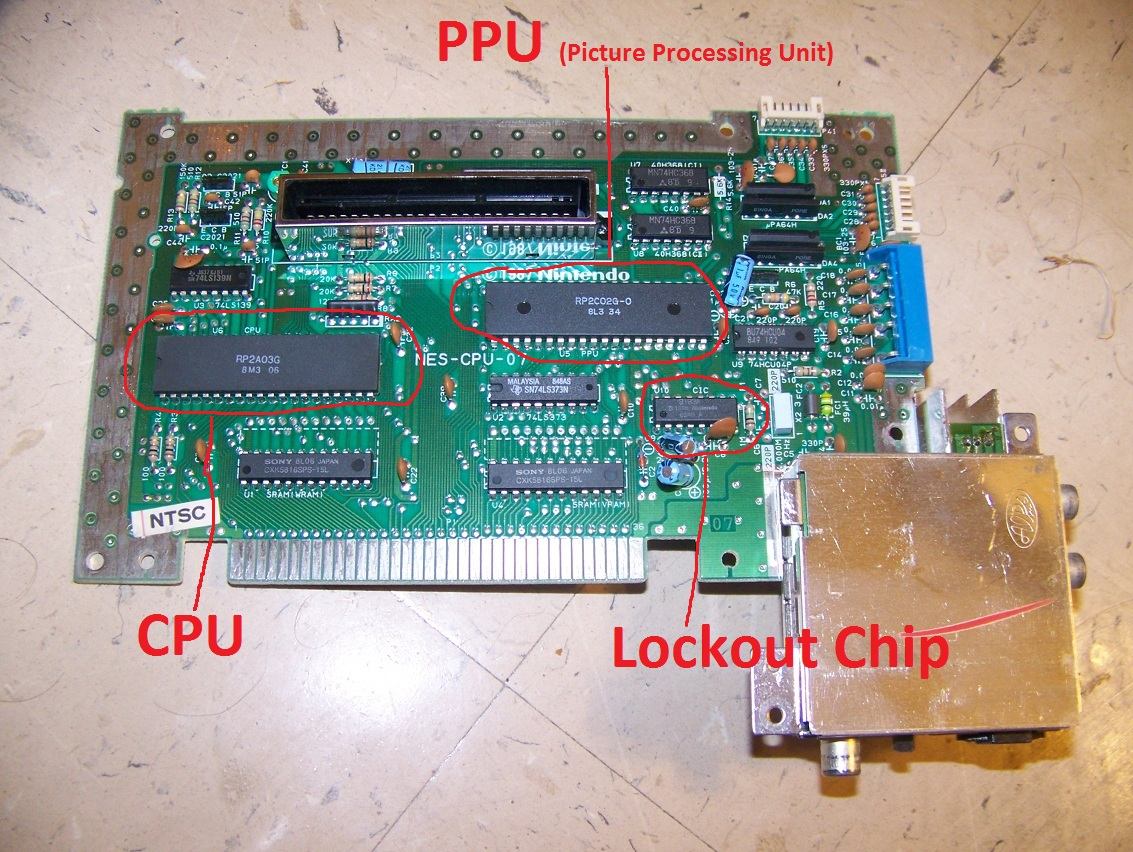
\includegraphics[width=\textwidth]{nes_motherboard}
		\end{column}
		\begin{column}{0.64\textwidth}
			\begin{itemize}
				\pause\item CPU: Ricoh 2A03 (closely based on MOS 6502)
				\pause\item Picture Processing Unit (PPU): Ricoh RP2C02 or RP2C07
				\pause\item RAM: 2 kilobytes for CPU + 2 kilobytes for PPU
				\pause\item Cartridge ROM: up to 1 megabyte, but typically less
				\pause\item Screen resolution: 256 $\times$ 240
			\end{itemize}
		\end{column}
	\end{columns}
\end{frame}

\begin{frame}{Technical limitations}
	\begin{itemize}
		\pause\item Around \textbf{2270 CPU cycles per frame}
		\pause\item Only \textbf{2 kilobytes} of writable memory to work with
		\pause\item 6502 instruction set is limited
			\begin{itemize}
				\pause\item 8-bit integer maths only
			\end{itemize}
		\pause\item The following are possible but need implementing as subroutines:
			\begin{itemize}
				\pause\item $>8$ bit numbers
				\pause\item Multiplication
				\pause\item Division
				\pause\item Fractional numbers
			\end{itemize}
	\end{itemize}
\end{frame}

\begin{frame}{Graphical limitations}
	\begin{itemize}
		\pause\item Display is made up of \textbf{sprites} and \textbf{background}
		\pause\item Sprites:
			\begin{itemize}
				\pause\item Maximum 64 on screen
				\pause\item Maximum 8 on the same scanline (horizontal line)
				\pause\item $8 \times 8$ pixels, 3 colours + transparency
				\pause\item Can flip horizontally or vertically
				\pause\item No rotation, scaling etc.
			\end{itemize}
		\pause\item Background:
			\begin{itemize}
				\pause\item Made of $8 \times 8$ pixel tiles
				\pause\item $32 \times 32$ blocks must share the same 4-colour palette
				\pause\item Limitations on types of scrolling
			\end{itemize}
	\end{itemize}
\end{frame}

\begin{frame}
	\begin{center}
		\url{https://wiki.nesdev.com/w/index.php/Limitations}
	\end{center}
\end{frame}

\begin{frame}{Examples of NES games}
	\begin{center}
		\url{https://youtu.be/um-GMygsRg4}
	\end{center}
\end{frame}

\begin{frame}{Designing your de-make}
	\begin{itemize}
		\pause\item Pitches \textbf{next week}!
		\pause\item Make sure you consider technical limitations carefully
	\end{itemize}
\end{frame}

